%# -*- coding: utf-8-unix -*-
%%==================================================
\chapter{题典之Hash}
\label{chap1}
\begin{itemize}[noitemsep,topsep=0pt,parsep=0pt,partopsep=0pt]
	\item 知识点:讲解相关知识点。
	\item 题型:直接上真题。
\end{itemize}

\section{知识点和方法论}

\subsection{知识点}

\begin{itemize}[noitemsep,topsep=0pt,parsep=0pt,partopsep=0pt]
	\item 开放定址法:H(key)为题目选定的散列函数, m 列表长度, di为增量序列, Hi新的位置
	\begin{itemize}[noitemsep,topsep=0pt,parsep=0pt,partopsep=0pt]
		\item 核心公式:$$ Hi = (H(key) + di) \% m $$ 
		\item 线性探测法: $$ di=0,1,2,3,...,m-1 $$
		\item 平方探测法(又称二次探测): $$ di=0,1,-1,4,-4,... k^2, -k^2 (k <= m / 2)$$
	\end{itemize}
    \item 平均查找长度
    \begin{itemize}[noitemsep,topsep=0pt,parsep=0pt,partopsep=0pt]
    	\item $$ ASL_{\mbox{成功} } = (\mbox{查找成功的次数,第一次也算一次}) / \mbox{元素的个数} $$ 
    \end{itemize}
	\item 平均失败查找长度
	\begin{itemize}[noitemsep,topsep=0pt,parsep=0pt,partopsep=0pt]
		\item $$ ASL_{\mbox{失败}} = ({\color{red}\mbox{在mod数范围内的空间才算}})/ {\color{red}\mbox{MOD后面的数}} $$ 
	\end{itemize}
	\item 装填因子: 衡量冲突的概率
	\begin{itemize}[noitemsep,topsep=0pt,parsep=0pt,partopsep=0pt]
		\item $$ \alpha = n(\mbox{关键字个数}) / N (\mbox{表长}) $$ 
	\end{itemize}
	\item 链地址法
	\begin{itemize}[noitemsep,topsep=0pt,parsep=0pt,partopsep=0pt]
		\item 就像领接表那样
	\end{itemize}
\end{itemize}

\subsection{方法论}
\begin{enumerate}[noitemsep,topsep=0pt,parsep=0pt,partopsep=0pt]
	\item 画出数组
	\item 后面填入数字(比较次数)
\end{enumerate}

\section{真题实战}


\subsection{2017年第8题}


\begin{lstlisting}[basicstyle=\small\ttfamily, caption={2017年第8题}, numbers=none]
已知Hash函数为H(K) = K mod 13 ,散列地址为0--14,用开放地址发解决冲突,选取增量序列为线性探测再散列,关键字
23,34,56,24,75,12,59,52,36,92 依次插入到散列表中,则平均成功的查找长度为____ 、  平均失败的查找长度为 _____。
\end{lstlisting}


解:


\begin{tabular}{|c|c|c|c|c|c|c|c|c|c|c|c|c|c|c|}% 通过添加 | 来表示是否需要绘制竖线
	\hline  % 在表格最上方绘制横线
	0 & 1 & 2 & 3 & 4 & 5 & 6 & 7 & 8 & 9 & 10 & 11 & 12 & 13 & 14 \\
	\hline  %在第一行和第二行之间绘制横线
	52(1) & 36(7) & 92(2) &   & 56(1) &   &   &   & 34(1) &   & 23(1) & 24(1) & 75(3) & 12(2) & 49(5) \\
	\hline
	 4 & 3 & 2 &  1 & 2 & 1 &  1 &  1 & 2 & 1 & 9 & 8 & 7 & 6 &  5  \\
	\hline % 在表格最下方绘制横线
\end{tabular}




\begin{lstlisting}[basicstyle=\small\ttfamily, caption={}, numbers=none]
23 % 13 = 10
34 % 13 = 8   
56 % 13 = 4
24 % 13 = 11
75 % 13 = 10  冲突  (10 + 1 ) % 15=11 冲突 (10 + 2)% 15 = 12
12 % 13 = 12  冲突  (12 + 1) % 15 =13 
49 % 13 = 10  冲突   (10 + 1 ) % 15=11 冲突 (10 + 2)% 15 = 12 冲突 (10 + 3) % 15 =13 冲突  (10 + 4) % 15 = 14
52 % 13 = 0 
36 % 13 = 10  冲突   (10 + 1 ) % 15=11 冲突 (10 + 2)% 15 = 12 冲突 (10 + 3) % 15 =13 冲突  (10 + 4) % 15 = 14 (10 + 5) % 15 = 0 冲突(10 + 6)% 15 = 1 
92 % 13 = 1 (1+1)% 15 = 2
\end{lstlisting}

\rule[-10pt]{20cm}{0.05em}

\begin{flalign}
1 + 7 + 2 + 1 + 1 + 1+ 1 + 3 + 2 + 5 &= 24  (\mbox{查找次数}) &&\\
24 / 10 &=2.4  (\mbox{平均查找长度}) 
\end{flalign}


对于0地址的元素要查找0,1,2,3这几个元素才知道会不会失败,第三个是空元素,所以失败了
对于1地址的元素要查找1,2,3这几个元素才知道会不会失败,第3个元素是空元素,所以失败了
以此类推
因为 mod 13 只用看  0 - 12空间里面的错误 
\begin{flalign}
(4+ 3 + 2 + 1 + 2 + 1 + 1 +1 + 2 + 1 + 9 + 8 + 7 ) &= 42 &&\\ 
ASL_{\mbox{失败}} &= 42 / 13 
\end{flalign}



\subsection{王道269综合应用题第3题}
\begin{figure}[htbp]
	\centering  % 环境中的内容居中排版
	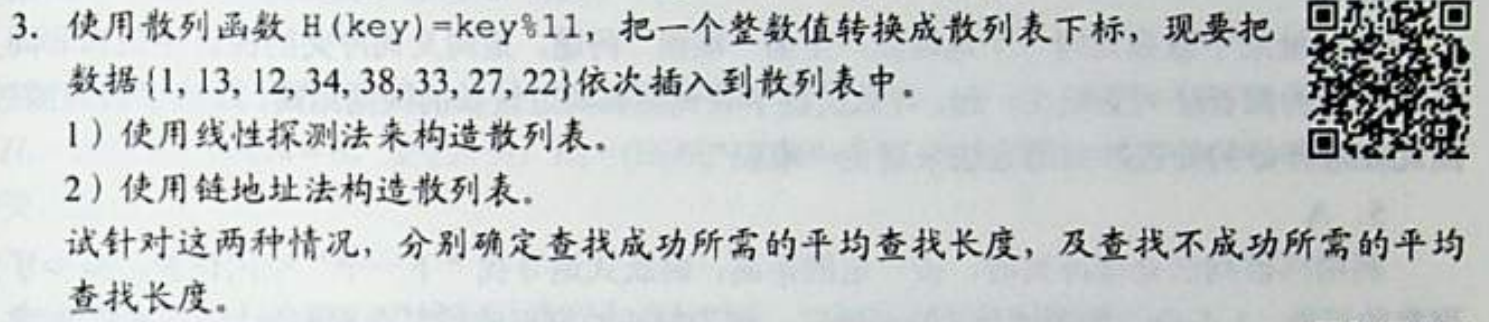
\includegraphics[scale=0.3]{example/chapter1/wangdao269_3.png}
	\caption{王道269综合应用题第3题}
\end{figure}


解:

1)
~\\
\begin{center}
\begin{tabular}{|c|c|c|c|c|c|c|c|c|c|c|}% 通过添加 | 来表示是否需要绘制竖线
	\hline  % 在表格最上方绘制横线
	0 & 1 & 2 & 3 & 4 & 5 & 6 & 7 & 8 & 9 & 10\\
	\hline  %在第一行和第二行之间绘制横线
	33(1) & 1(1) & 13(1) & 12(3) & 34(4) & 38(1)  & 27(2) & 22(8)  &  &   &  \\
	\hline % 在表格最下方绘制横线
\end{tabular}
\end{center}
~\\

\begin{lstlisting}[basicstyle=\small\ttfamily, caption={}, numbers=none]
1 % 11 = 1 
13 % 11 = 2
12 % 11 = 1冲突   (1+1)% 10 = 2 冲突   (1  + 2) % 10 = 3
34 % 11 = 1冲突   (1+1)% 10 = 2 冲突   (1  + 2) % 10 = 3 冲突(1+ 3) % 10 = 4 
33 % 11 = 0
38 % 11 = 5
27 % 11 = 5 冲突 (5+1)%10 = 6
22 % 11 = 0 冲突  1 冲突 2 冲突3 冲突4 冲突5 冲突 6冲突   7
\end{lstlisting}
~\\
2)
\\~
拉链法只要算一次
\begin{lstlisting}[basicstyle=\small\ttfamily, caption={}, numbers=none]
1 % 11 = 1 
13 % 11 = 2
12 % 11 = 1
34 % 11 = 1 
33 % 11 = 0
38 % 11 = 5
27 % 11 = 5 
22 % 11 = 0 
\end{lstlisting}

\begin{figure}[H]
	\centering  % 环境中的内容居中排版
	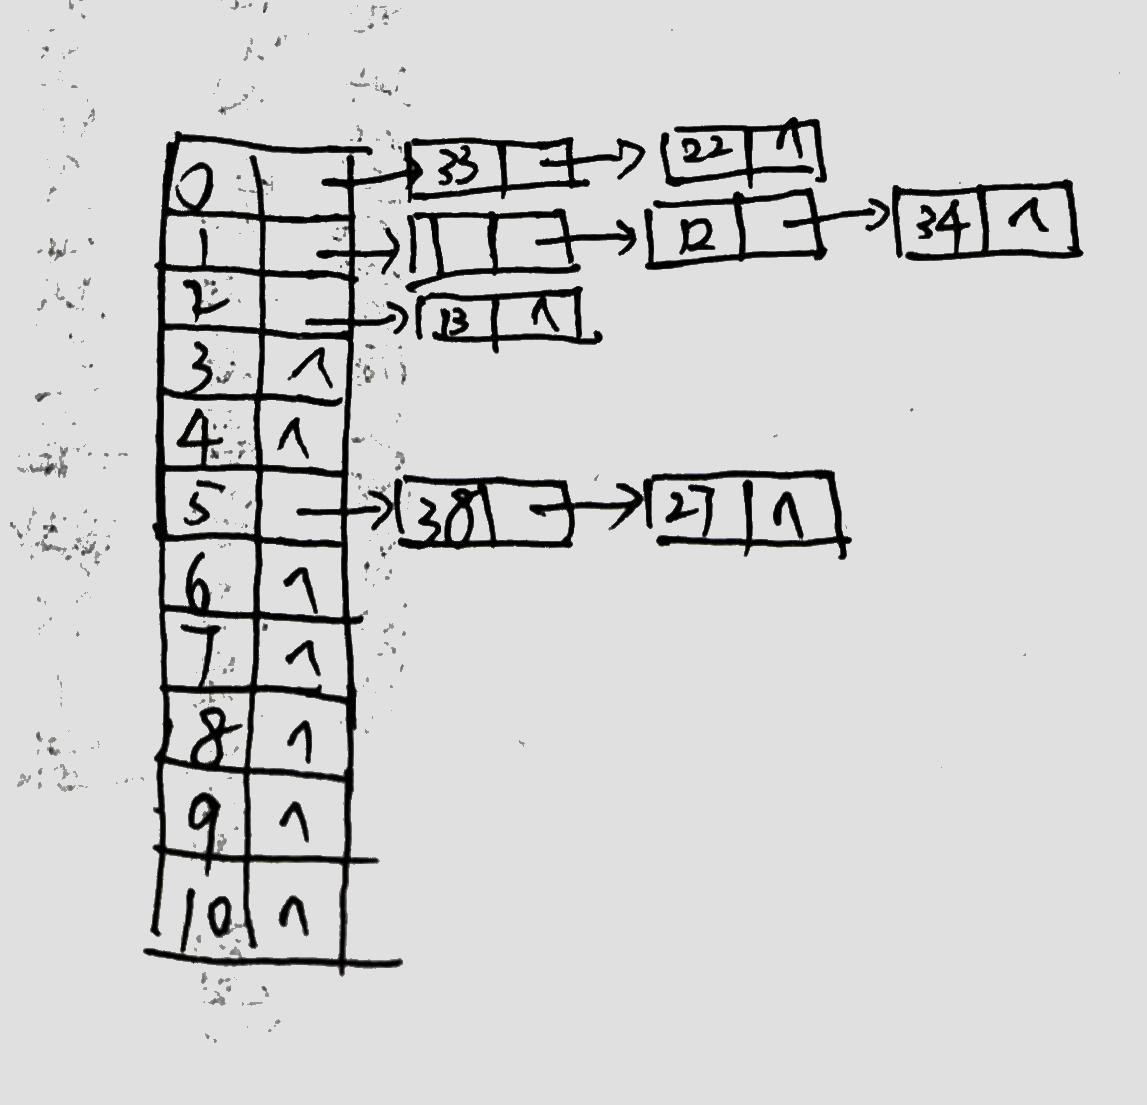
\includegraphics[scale=0.3]{example/chapter1/lalianfa.jpg}
	\caption{王道269综合应用题第3题}
\end{figure}

3)
\\~
\begin{lstlisting}[basicstyle=\small\ttfamily, caption={}, numbers=none]
用A B 指代 1) 2)
A
A(ASL 成功) = (1+ 1 + 1 + 3 + 4 + 1 + 2 + 8)/8=21 / 8
A(ASL 失败) = (9 + 8 + 7 + 6 + 5 + 4 + 3 + 2 + 1 + 1 + 1) / 11 = 47 / 11
B
B(ASL成功) = (4*1 + 3*2 + 3 * 1)/8 = 13 / 8
B(ASL失败) = (3 + 4 + 2 + 1 + 1 + 3 + 1*5) / 11 = 19 / 11
\end{lstlisting}


\subsection{2015年第(5)题}


\begin{lstlisting}[basicstyle=\small\ttfamily, caption={}, numbers=none]
设散列函数 H(K) = 3K mod 11, 散列地址空间为 0 - 10, 对关键字序列 (32,13,39,24,38,21,4,12) 按照下述两种解决冲突的方法构造散列表;
1) 线性探测再散列;
2) 链地址法;
3) 并分别求出等概率下查找成功时和查找失败时的平均查找长度 ASL_{succ} 和 ASL_{UNSUCC};
\end{lstlisting}
解:
\\~
\begin{center}
\begin{tabular}{|c|c|c|c|c|c|c|c|c|c|c|}% 通过添加 | 来表示是否需要绘制竖线
	\hline  % 在表格最上方绘制横线
	0 & 1 & 2 & 3 & 4 & 5 & 6 & 7 & 8 & 9 & 10\\
	\hline  %在第一行和第二行之间绘制横线
	& 4(1) &   & 49(1) & 38(1) & 12(3)  & 13(1) & 24(2)  & 32(1) & 21(2)  &   \\
	\hline % 在表格最下方绘制横线
\end{tabular}
\end{center}

\begin{lstlisting}[basicstyle=\small\ttfamily, caption={}, numbers=none]
(3*32) % 11 = 8
(13*3) % 11 = 6   
(49*3) % 11 = 3
(24*3) % 11 = 6 冲突 (6+1) %11 = 7
(38*3) % 11 = 4
(21*3) % 11 = 8 冲突 (8+1) %11 = 9
(4*3)  % 11 = 1
(12*3) % 11 = 3 冲突  4 冲突  5
\end{lstlisting}
~\\
\begin{flalign}
ASL_{\mbox{失败}} &= (1+2+8+7+6+5+4+3+2+1) / 11 =  39/11 &&\\ 
ASL_{\mbox{成功}} &= (1+1+1+3+1+2+1+2) / 8 = 1.5
\end{flalign}
\\~
\begin{flalign}
ASL_{\mbox{失败}} &= (1+2+1+3+2+1+3+1+3+1+1) / 11 =  19/11 &&\\ 
ASL_{\mbox{成功}} &= (5*1 + 3*2) / 8 = 11 / 8 
\end{flalign}


\subsection{2013年第4题}


\begin{lstlisting}[basicstyle=\small\ttfamily, caption={}, numbers=none]
设哈希函数为H(key) = key mod 13 哈希表长为15,用开放定址法处理冲突,增量序列使用二次探测再散列。若一次在哈希表中插入11个元素:
34,12,67,43,98,23,51,86,05,37,22
1) 画出他们在表中的分布情形。
2) 求其等概率情况下平均成功的查找长度
\end{lstlisting}

解:

\begin{center}
\begin{tabular}{|c|c|c|c|c|c|c|c|c|c|c|c|c|c|c|}% 通过添加 | 来表示是否需要绘制竖线
	\hline  % 在表格最上方绘制横线
	0 & 1 & 2 & 3 & 4 & 5 & 6 & 7 & 8 & 9 & 10 & 11 & 12 & 13 & 14 \\
	\hline  %在第一行和第二行之间绘制横线
	&  & 67(1) & 22(6) & 43(1) & 5(1)  &   &  98(1) & 34(1) & 86(2)  & 23(1) & 37(1) & 12(1) & 51(2) &  \\
	\hline % 在表格最下方绘制横线
\end{tabular}
\end{center}
~\\
\begin{lstlisting}[basicstyle=\small\ttfamily, caption={}, numbers=none]
39 % 13 = 8
12 % 13 = 12
67 % 13 = 2
43 % 13 = 4
98 % 13 = 7
23 % 13 = 10
51 % 13 = 12 冲突 (12+1) % 15 = 13
86 % 13 = 8 冲突 (8+1) % 15 = 9
5 % 13 =5
37 % 13 = 11
22 % 13 = 9 冲突 (9+1) %15 = 10 冲突 (9-1)%15 = 8 冲突 (9+4) %15 = 13 冲突 (9-4) %15 = 5 冲突 (9+9) %15 = 3
\end{lstlisting}
~\\
\begin{flalign}
ASL_{\mbox{成功}} &= (1+6+1=1+1+1+2+1+1+1+2) / 11 = 18/11
\end{flalign}


\subsection{2014年第4题}
\begin{lstlisting}[basicstyle=\small\ttfamily, caption={}, numbers=none]
采用哈希后函数H(k) = 3*k mod 13 并用开放地址发处理冲突,增量序列选取采用线性探测再散列方式,在数列地址空间[0..12]中对关键字序列
22,41,53,46,30,13,1,67,51
1) 构造哈希表(画示意图);
2) 装填因子;
3) 查找成功时的平均查找长度;
4) 查找不成功时的平均查找长度。
\end{lstlisting}
解:
~\\
\begin{center}
\begin{tabular}{|c|c|c|c|c|c|c|c|c|c|c|c|c|}% 通过添加 | 来表示是否需要绘制竖线
	\hline  % 在表格最上方绘制横线
	0 & 1 & 2 & 3 & 4 & 5 & 6 & 7 & 8 & 9 & 10 & 11 & 12  \\
	\hline  %在第一行和第二行之间绘制横线
	13,1& 66,1 &  & 53,1 & 1,2 &   & 41,1  &  67,2 & 46,1 &   & 51,1 &  & 30,1   \\
	\hline % 在表格最下方绘制横线
\end{tabular}
\end{center}
~\\
\begin{lstlisting}[basicstyle=\small\ttfamily, caption={}, numbers=none]
3*22 % 13 = 1
41*3 % 13 = 6
53*3 % 13 = 3
46*3 % 13 = 8
30*3 % 13 = 12
13*3 % 13 = 0
(1*3)% 13 = 3 冲突 4
(667*3)%13 = 6 冲突 7
(51*3) %13 = 10
\end{lstlisting}
~\\
\begin{flalign}
\alpha = \frac{n}{N} = \frac{9}{13}
\end{flalign}
~\\
\begin{flalign}
ASL_{\mbox{成功}} &= (1+1+1+2+1+2+1+1+1) / 9 = 11/9 &&\\
ASL_{\mbox{失败}} &= (3+2+1+3+2+1+4+3+2+1+2+1+4) / 13 = 29/13 
\end{flalign}



